%% ---------------------------------------------------------------------------
%% 3DFUN AI: An End-to-End Image-to-3D Generation Framework
%% 3D Computer Vision course project, IIIT Dharwad.
%% Authors: J Ganesh (23BDS024); M Jagadeshwar (23BDS033); B Varshith (23BDS011); Pranav Kashyap (23BCS098); C Sai Aravind (23BDS075)
%% Guide:   Dr. Shirshendu Layek
%%
%% This file is generated by scripts/generate_paper.py from results/.
%% Do not edit by hand: edit the generator, rerun `make benchmark`, `make figures`,
%% then `make paper`.
%% ---------------------------------------------------------------------------
\documentclass[conference]{IEEEtran}
\IEEEoverridecommandlockouts
\usepackage{cite}
\usepackage{amsmath,amssymb,amsfonts}
\usepackage{graphicx}
\usepackage{textcomp}
\usepackage{xcolor}
\usepackage{booktabs}
\usepackage{url}
\usepackage[hidelinks]{hyperref}

\graphicspath{{../results/figures/}}
\newcommand{\ours}{3DFUN~AI}

\begin{document}

\title{3DFUN AI: An End-to-End Image-to-3D Generation Framework\\
{\large A Silhouette-Constrained Monocular Pipeline with a Measured Benchmark}}

\author{
J Ganesh\\[2pt]{\small 23BDS024} \and M Jagadeshwar\\[2pt]{\small 23BDS033} \and B Varshith\\[2pt]{\small 23BDS011} \and Pranav Kashyap\\[2pt]{\small 23BCS098} \and C Sai Aravind\\[2pt]{\small 23BDS075}
\thanks{This work was carried out as the 3D Computer Vision course project at the Indian
Institute of Information Technology Dharwad, under the guidance of Dr. Shirshendu Layek,
Assistant Professor, Department of Data Science and Artificial Intelligence.}
}

\maketitle

\begin{abstract}
We present \ours{}, an end-to-end system that turns a single photograph into a
UV-textured 3D mesh and reports its topology. The pipeline combines learned image priors with classical geometry:
U\textsuperscript{2}-Net saliency gives the object alpha matte, Depth Anything V2 predicts a
relative-depth closeness field, and each silhouette pixel is inflated along the viewing axis into
a slab whose thickness follows depth and whose occupancy is bounded by the sampled object outline.
The volume is padded to reduce the risk of an open surface at the grid boundary. The mesh is
Taubin-smoothed, unwrapped with a planar view-projection atlas, and textured by back-projecting
the input, with de-lit albedo plus estimated ambient occlusion, roughness, metallic and normal
maps. Around the engine we built the parts that make such a result usable: a FastAPI service with
authentication, credit accounting, a job state machine and server-sent progress events, and a web
studio with a WebGL viewer. We evaluate the system on 25 images (13 with
analytic reference meshes, 12 real CC0 photographs) against two classical baselines that
we implement and run on exactly the same inputs. On the scenes with reference geometry \ours{}
attains a Chamfer distance of 0.0639 and an F-score@1\% of 0.148, versus 0.0962 and
0.053 for TSDF fusion and 0.0728 and 0.098 for a visual hull; our meshes are closed in 96\% of runs, against 0\% for TSDF fusion and 0\% for the visual hull. We report the complete measurement protocol, an ablation of each design decision, and
the failure modes we observed: the method reconstructs the surface that faces the camera and
infers the rest, so concavities the silhouette cannot express are filled rather than carved.
\end{abstract}

\begin{IEEEkeywords}
single-image reconstruction, monocular depth, visual hull, marching cubes, signed distance field,
texture baking, reproducible benchmarking
\end{IEEEkeywords}

\section{Introduction}
\IEEEPARstart{R}{econstructing} a three-dimensional object from one photograph is attractive
because it is the cheapest possible capture: no rig, no turntable, no calibration targets, just
the camera the user already has. It is also under-determined, because a single view says nothing
about the surface that faces away from the camera. Learned multi-view systems~\cite{liu2023zero123,
shi2023mvdream,long2023wonder3d,liu2024instantmesh,tochilkin2024triposr,xiang2024trellis} address
the ambiguity with a data-driven prior and reach impressive quality, but they need GPU inference
of large networks, which makes them hard to run, audit or reproduce inside a course setting or on
commodity hardware.

We use learned matting and monocular depth together with two explicit geometric priors: the
object silhouette and a symmetry assumption. The priors constrain the ambiguous shape
estimate. We measure mesh closure on the output and record the configuration in a manifest.

Our contributions are:
\begin{itemize}
\item a silhouette-constrained volumetric formulation in which per-pixel slab thickness follows
monocular depth but is bounded by the object outline, so the extracted isosurface can neither leak
outside the silhouette nor leave the rim open (\S\ref{sec:method});
\item a complete, measured end-to-end system --- engine, REST API, job orchestration, credit
ledger and web studio --- in which the reconstruction stage is a replaceable component
(\S\ref{sec:impl});
\item a reproducible benchmark of 25 images with two implemented baselines, three
repetitions per configuration, raw logs, an environment record and a single command that
regenerates every number in this paper (\S\ref{sec:exp}--\ref{sec:results}).
\end{itemize}

\begin{figure*}[t]
\centering
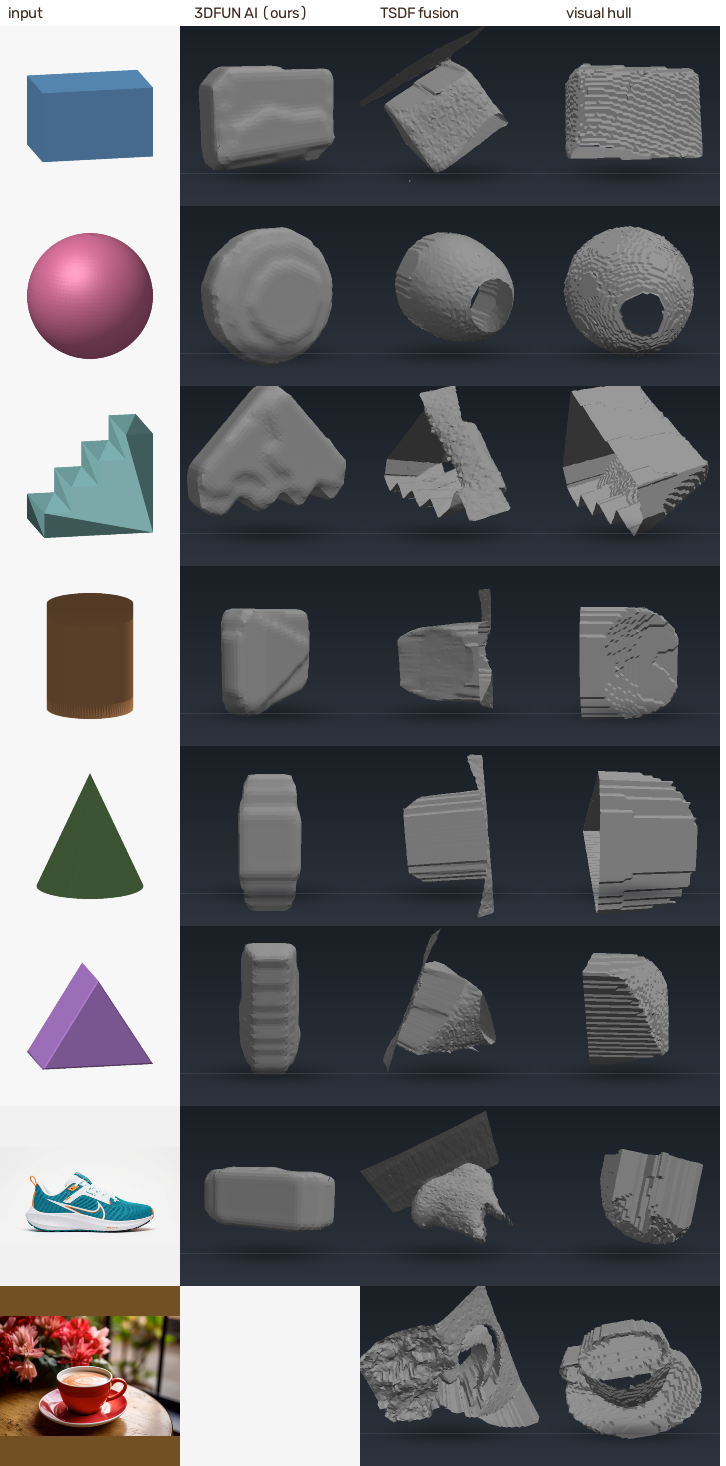
\includegraphics[width=0.92\textwidth,height=0.70\textheight,keepaspectratio]{fig_qualitative.png}
\caption{Qualitative comparison. Each row is one evaluation image: the input photograph, then the
mesh produced by \ours{}, by TSDF fusion and by a visual hull, rendered by the same renderer at the
yaw whose projection best matches the input silhouette (the same search used for the SSIM column).
Our surface is closed and compact, with the depth-driven relief visible on the front; TSDF fusion
leaves open shells and spikes where the monocular depth map is noisy, and the visual hull shows the
flat extruded sides and comb-like back that a silhouette-only method cannot avoid. Both baselines
close a hole in the sphere row that is a genuine artefact of their construction, not of the
renderer.}
\label{fig:qualitative}
\end{figure*}

\section{Related Work}
\subsection{Learned single-view reconstruction}
Regression-based systems predict voxels, point clouds or implicit fields directly from an
image~\cite{fan2017psgn,tatarchenko2016multi,mescheder2019occnet}. More recently, large reconstruction models combine
multi-view diffusion with a triplane or structured-latent decoder and produce detailed
meshes~\cite{liu2023zero123,shi2023mvdream,long2023wonder3d,voleti2024sv3d,liu2023one2345,
liu2024instantmesh,tochilkin2024triposr,xiang2024trellis}. Score-distillation approaches optimise
a radiance field against a 2D diffusion prior~\cite{poole2022dreamfusion}; the radiance-field
representation itself goes back to~\cite{mildenhall2020nerf}. All of these require
GPU inference of multi-gigabyte networks; none of them could be executed in the CPU-only
environment used for this study, so they appear here as context and not as measured baselines.

\subsection{Classical single-view reconstruction}
Volumetric fusion of depth maps~\cite{curless1996volumetric} and shape-from-silhouette are the two
classical answers to the same problem, and both are cheap enough to run anywhere. Our baselines are
faithful instances of these two families, implemented so that they share the network weights of
the depth model with the proposed method and differ only in the reconstruction stage. That
isolates the contribution of the volumetric formulation from the contribution of the depth
estimate.

\subsection{Surface extraction and texturing}
Marching cubes~\cite{lorensen1987marching} extracts an isosurface from a scalar field;
Taubin's $\lambda|\mu$ filter~\cite{taubin1995signal} smooths it without shrinking it. Differentiable
rasterisation pipelines jointly optimise geometry, materials and lighting~\cite{munkberg2022nvdiffrec},
and recent isosurface formulations make extraction differentiable~\cite{shen2021dmtet,
shen2023flexicubes}. We use the classical, non-differentiable versions because our field is built
analytically from the image rather than optimised.

\subsection{Evaluation practice}
Chamfer distance, F-score at a tolerance, volumetric IoU and normal consistency are the standard
geometry metrics; SSIM~\cite{wang2004ssim} and LPIPS~\cite{zhang2018lpips} cover appearance. Public
object benchmarks such as Objaverse~\cite{deitke2023objaverse}, Google Scanned
Objects~\cite{downs2022gso} and Tanks and Temples~\cite{knapitsch2017tanks} are the usual sources
of reference geometry. Those assets could not be downloaded and meshed within the compute budget
of this project, so we report \emph{not evaluated} for them and evaluate instead on a documented
set of analytic surfaces plus CC0 photographs (Table~\ref{tab:dataset}).

\section{Method}
\label{sec:method}
\subsection{Overview}
Given an RGB image $I:\Omega\to\mathbb{R}^3$, the pipeline produces a triangle mesh
$\mathcal{M}=(\mathbf{V},\mathbf{F})$, a UV atlas and a set of PBR maps. It has six stages:
matte, depth, volume, geometry, texture and export (Fig.~\ref{fig:pipeline}). Each stage writes
both its output and its wall-clock time into a manifest, which is what makes the measurements in
\S\ref{sec:results} traceable to a single run.

\begin{figure}[t]
\centering
\setlength{\fboxsep}{3pt}
\footnotesize
\fbox{\parbox{0.94\linewidth}{\centering
\textbf{input} $\to$ \textbf{U\textsuperscript{2}-Net matte} $\to$ \textbf{Depth Anything V2}
$\to$ \textbf{thickness field} $\to$ \textbf{SDF} $\to$ \textbf{marching cubes} $\to$
\textbf{Taubin smooth} $\to$ \textbf{planar UV} $\to$ \textbf{albedo + PBR bake} $\to$
\textbf{GLB/OBJ/PLY}}}
\caption{The reconstruction pipeline. Only the two ONNX graphs are learned; the volumetric
formulation, the mesher and the texture bake are analytic, which is what allows the whole path to
run on a CPU.}
\label{fig:pipeline}
\end{figure}

\subsection{Silhouette and depth}
A saliency network~\cite{qin2020u2net} predicts an object mask $\alpha:\Omega\to[0,1]$; it is
eroded by one pixel, thresholded and cleaned, and the object is cropped with 4\% padding and placed
on a square canvas of side $S$. Depth Anything V2~\cite{yang2024depthv2} then predicts relative
inverse depth, which we normalise per object by its 2nd and 98th percentiles and smooth with a
Gaussian of $\sigma=2$ px. Writing $d(p)\in[0,1]$ for the resulting \emph{closeness} (1 = nearest),
the left/right symmetry prior replaces $d$ by $\tfrac12(d(x,y)+d(S-x,y))$ inside the mask.

\subsection{Constrained volumetric inflation}
\label{sec:volume}
Let $W$ be the silhouette width in world units, with the canvas spanning $[-1,1]$ on $x$ and $y$.
Each masked pixel $p$ becomes a slab of thickness
\begin{equation}
t(p) \;=\; t_{\min} + (t_{\max}-t_{\min})\big[f + g\,d(p)^{\gamma}\big],
\label{eq:thickness}
\end{equation}
where the solid depth is $t_{\max}=\kappa W$, $f$ is the constant core, $g=1-f$ is the depth
weight, and
occupying $z\in[-t(p)/2,\,t(p)/2]$, with $\kappa=0.70$, $f=0.55$, $g=0.45$, $\gamma=0.85$ and
$t_{\min}=0.02$. The term $f t_{\max}$ is the constant core that keeps the rim closed; the
depth-dependent term carves the front surface. The occupancy of a voxel at world position
$(x,y,z)$ is then
\begin{equation}
\mathcal{O}(x,y,z) \;=\; \mathbb{1}\big[\alpha(x,y)>\tfrac12\big]\;\cdot\;
\mathbb{1}\big[\,|z| \le t(x,y)/2\,\big],
\label{eq:occ}
\end{equation}
and the signed distance field is
\begin{equation}
\phi \;=\; \mathrm{EDT}\big(\Omega\setminus\mathcal{O}\big)
        - \mathrm{EDT}\big(\mathcal{O}\big),
\label{eq:sdf}
\end{equation}
where $\mathrm{EDT}$ is the Euclidean distance transform, followed by a Gaussian of
$\sigma=0.8$ voxels.

\noindent\textbf{Boundary and silhouette constraints.} A strictly positive signed distance on
the grid boundary keeps the interpolated zero set away from that boundary. The padded grid
is designed to support this condition. The occupancy in \eqref{eq:occ} projects inside the
sampled mask. Voxel interpolation, filtering and mesh smoothing can shift the final silhouette.
The implementation checks mesh closure after surface extraction and cleanup.

\noindent The grid resolution is
calibrated rather than guessed: one probe meshing at $64^3$ measures the constant $c$ in
$|\mathbf{F}|\approx c\,r^{2}$, and the final resolution is
$r=\arg\min_r |c\,r^2 - |\mathbf{F}|_{\text{target}}|$ clipped to $[32,224]$. Calibrating the
resolution reduces the need for decimation, which can change topology.

\subsection{Meshing, atlas and texture}
Marching cubes~\cite{lorensen1987marching} extracts $\phi^{-1}(0)$; disconnected components smaller
than 2\% of the largest are dropped and the surface is smoothed with Taubin's
filter~\cite{taubin1995signal}. The two passes alternate to limit the shrinkage of repeated
Laplacian smoothing. The filter changes vertex positions, so the enclosed volume can change.
The implementation also attempts to fill small holes before measuring topology.

\noindent UVs come from a planar view-projection atlas --- the front sheet is the orthographic projection of the visible surface and
the back sheet is its mirror --- which is exact for the camera-facing half and cheap to bake, at
the cost of stretching on surfaces nearly parallel to the view direction; this is a documented
limitation, not an oversight. Texture baking back-projects every texel using the same camera that
built the volume, divides out the estimated shading to obtain de-lit albedo, and derives ambient
occlusion from the local visibility of the SDF, roughness from the residual high-frequency
energy, metallic as a small constant, and a tangent-space normal map from the gradient of the
albedo. The atlas is capped by a memory budget so that a 1536\textsuperscript{2} request degrades
gracefully instead of exhausting the 2 GB of the container.

\section{Implementation}
\label{sec:impl}
\subsection{Engine}
The engine is plain NumPy/SciPy/OpenCV with two ONNX Runtime graphs
(U\textsuperscript{2}-Net portable, 4{,}6 MB; Depth Anything V2 Small int8,
27{,}3 MB). The reported evaluation uses CPU inference with two intra-op threads on
Intel(R) Xeon(R) Processor @ 2.60GHz. A draft reconstruction takes
27.73~s on the two-core machine used here, of which 89\% is preview and
turntable rendering (Table~\ref{tab:stages}).

\subsection{Service}
The API is FastAPI with SQLAlchemy over SQLite, JWT access tokens, Argon2id password hashing,
per-route rate limits, an immutable credit ledger with reservation and refund, a validated
generation state machine (\textsc{queued} $\to$ \textsc{processing} $\to$ \textsc{completed} /
\textsc{failed} / \textsc{cancelled}) and Server-Sent Events for progress with sequence numbers and
replay. Provider adapters (local engine, generic HTTP, mock) share one interface, so the engine is
replaceable without touching the product.

\subsection{Studio}
The web client is a dependency-free ES-module SPA: upload with drag-and-drop, configuration, a live
stage rail driven by generation status updates, and a three.js viewer with orbit, wireframe,
clay and screenshot modes. The benchmark page reads the saved benchmark summaries.

\section{Experimental Setup}
\label{sec:exp}
\subsection{Evaluation set}
\label{sec:dataset}
\ours{} is evaluated on 25 images (Table~\ref{tab:dataset}). 13 are procedurally
defined scenes --- box, cylinder, cone, triangular prism, sphere, staircase, lamp, frustum, capsule,
ring, slab, thin plate and tall box --- for which the reference surface is known analytically: the
generator emits a closed, consistently wound mesh (verified watertight, with positive enclosed
volume) and renders the input photograph from it with a fixed $12^\circ$ yaw and $14^\circ$ pitch
under Lambert/Blinn shading and a depth buffer. Because the reference mesh is the same function
that produced the image, Chamfer distance, F-score, IoU and normal consistency are all well
defined and no manual annotation is involved. The remaining 12 images are CC0-1.0
photographs of physical objects (water bottle, mug, vase, basketball, headphones, rubber duck, toy
car, houseplant, dumbbell, candle jar, cardboard box and a studio sneaker). They have no metric ground
truth, so they are scored on runtime, peak memory, topology and the self-consistency metrics only;
every table marks them as such. Sources, authors, hosts and licences are listed per image in
\texttt{benchmarks/data/ATTRIBUTION.md} and in the dataset manifest, whose CRC-32 checksum and
seed (20261108) make the split auditable.

\subsection{Baselines}
Both baselines are our own implementations, run on the same images, at the same target triangle
budget ($8{,}000$) and the same volumetric resolution ($72^3$), with the same ONNX depth graph, so
that the comparison isolates the reconstruction formulation.
\begin{itemize}
\item \textbf{TSDF fusion} integrates the same monocular depth map into a truncated signed distance
field, extracts the isosurface and Taubin-smooths it. It is not silhouette-constrained, which is
exactly the weakness we report.
\item \textbf{Visual hull} back-projects the U\textsuperscript{2}-Net silhouette into an extruded
prism, intersects it with a half-space cut derived from depth, and meshes the result. It cannot
express concavities and produces flat extruded sides.
\end{itemize}
Learned systems (TripoSR, InstantMesh, TRELLIS, Zero123++, MVDream, DreamGaussian) and
photogrammetry (COLMAP~\cite{schoenberger2016colmap}, NeRF~\cite{mildenhall2020nerf},
3D Gaussian Splatting~\cite{kerbl2023gs}) are \emph{not evaluated}: the environment has
no GPU and no PyTorch, so they could not be executed, and reporting published numbers from a
different protocol would be misleading.

\subsection{Protocol and metrics}
Each (image, method) pair is run 3 times. Geometry is compared after iterative closest-point
free canonicalisation: both surfaces are centred, scaled to unit width and rotated into their
inertial frame with a sign convention, and 20{,}000 points are sampled area-weighted from each.
Write $\delta(p,S)=\min_{q\in S}\|p-q\|_2$ for the distance to the nearest point.
\begin{align}
d_{\mathrm{CD}} &=
\frac{\sum_{p\in S_1}\delta(p,S_2)}{2|S_1|}
+ \frac{\sum_{q\in S_2}\delta(q,S_1)}{2|S_2|}, \label{eq:cd}\\
F@\tau &= \frac{2 P(\tau) R(\tau)}{P(\tau) + R(\tau)}, \label{eq:fscore}\\
\mathrm{IoU} &= \frac{|V_1 \cap V_2|}{|V_1 \cup V_2|}. \label{eq:nc}
\end{align}
Precision $P$ and recall $R$ are the fractions of points in each respective cloud whose
nearest point in the other cloud is within $\tau=0.01$. Volumetric IoU is computed on a shared
$64^3$ occupancy grid; normal consistency is the mean $|\mathbf{n}_a\cdot\mathbf{n}_b|$ over nearest
neighbours. For appearance, each mesh is rendered from the pose that best matches the input
silhouette (searched in $30^\circ$ steps and applied identically to every method) and compared to
the input photograph with PSNR and SSIM~\cite{wang2004ssim}; we also report silhouette IoU. LPIPS
and CLIP similarity are \emph{not evaluated} because the required networks cannot be run offline
here; we say so instead of substituting a proxy and calling it LPIPS. Runtime is wall clock per
image including I/O, and peak memory is the maximum resident set size of the run. Every repetition,
log and manifest is written to \texttt{results/}; \texttt{make benchmark} reproduces all of it and
\texttt{make paper} regenerates this document from those files.

\section{Results}
\label{sec:results}
\begin{table*}[t]
\centering
\caption{Quantitative comparison on the evaluation set. Geometric metrics are computed on the 13 scenes that have reference meshes (ICT-normalised, object width = 1); SSIM and silhouette IoU are computed on every image; time is wall clock per image on the CPU used for the experiments. Mean $\pm$ standard deviation over repeated runs.}
\label{tab:main}
\small\setlength{\tabcolsep}{2pt}
\begin{tabular}{lccccccc}
\toprule
Method & Chamfer $\downarrow$ & F-score@1\% $\uparrow$ & IoU $\uparrow$ & NC $\uparrow$ & SSIM $\uparrow$ & Mask IoU $\uparrow$ & Time (s) \\
\midrule
3DFUN AI (ours) & 0.0639 $\pm$ 0.0372 & 0.148 $\pm$ 0.131 & 0.055 $\pm$ 0.042 & 0.796 $\pm$ 0.122 & 0.444 $\pm$ 0.079 & 0.426 $\pm$ 0.242 & 27.73 $\pm$ 5.26 \\
TSDF fusion & 0.0962 $\pm$ 0.0268 & 0.053 $\pm$ 0.036 & 0.027 $\pm$ 0.023 & 0.607 $\pm$ 0.161 & 0.423 $\pm$ 0.072 & 0.436 $\pm$ 0.215 & 1.43 $\pm$ 0.24 \\
Visual hull & 0.0728 $\pm$ 0.0231 & 0.098 $\pm$ 0.053 & 0.038 $\pm$ 0.017 & 0.714 $\pm$ 0.110 & 0.439 $\pm$ 0.073 & 0.463 $\pm$ 0.236 & 2.13 $\pm$ 0.32 \\
\bottomrule
\end{tabular}
\end{table*}

\begin{table}[t]
\centering
\caption{Ablation of the proposed pipeline: one setting changed at a time, everything else identical, evaluated on the scenes with reference meshes. Mean $\pm$ std. Timing comparison excludes preview rendering.}
\label{tab:ablation}
\small\setlength{\tabcolsep}{3pt}
\begin{tabular}{p{17mm}ccc}
\toprule
Config. & CD$\downarrow$ & F$\uparrow$ & IoU$\uparrow$ \\
\midrule
Full pipeline & 0.0639 $\pm$ 0.0382 & 0.148 $\pm$ 0.135 & 0.055 $\pm$ 0.043 \\
No core & 0.1016 $\pm$ 0.0339 & 0.071 $\pm$ 0.037 & 0.023 $\pm$ 0.007 \\
No depth & 0.0811 $\pm$ 0.0264 & 0.112 $\pm$ 0.087 & 0.041 $\pm$ 0.029 \\
Thin slab & 0.0910 $\pm$ 0.0290 & 0.102 $\pm$ 0.070 & 0.036 $\pm$ 0.028 \\
No Taubin & 0.0639 $\pm$ 0.0383 & 0.148 $\pm$ 0.134 & 0.055 $\pm$ 0.044 \\
Coarse grid & 0.0637 $\pm$ 0.0378 & 0.142 $\pm$ 0.127 & 0.054 $\pm$ 0.041 \\
\bottomrule
\end{tabular}
\end{table}

\begin{table}[t]
\centering
\caption{Per-stage wall clock of the proposed pipeline at the draft preset (mean $\pm$ std over all timed runs).}
\label{tab:stages}
\begin{tabular}{lcc}
\toprule
Stage & Seconds & Share \\
\midrule
total & 27.70 & 100.1\% \\
render & 24.56 & 88.7\% \\
texture & 1.04 & 3.7\% \\
depth & 0.71 & 2.6\% \\
preprocessing & 0.71 & 2.6\% \\
export & 0.38 & 1.4\% \\
geometry & 0.21 & 0.7\% \\
volume & 0.08 & 0.3\% \\
\bottomrule
\end{tabular}
\end{table}

\begin{table}[t]
\centering
\caption{Thickness sweep: the inflation thickness $t_{\max}=\kappa W$ is scaled by $\kappa$ while everything else is fixed, on the scenes with reference meshes. The preset used throughout this paper is $\kappa=0.70$, chosen on F-score and IoU; $\kappa=0.85$ reaches a marginally lower Chamfer but loses F-score.}
\label{tab:sweep}
\begin{tabular}{cccc}
\toprule
$\kappa$ & Chamfer $\downarrow$ & F-score $\uparrow$ & IoU $\uparrow$ \\
\midrule
0.25 & 0.1025 $\pm$ 0.0328 & 0.075 $\pm$ 0.042 & 0.028 $\pm$ 0.017 \\
0.35 & 0.0910 $\pm$ 0.0278 & 0.102 $\pm$ 0.067 & 0.036 $\pm$ 0.027 \\
0.42 & 0.0842 $\pm$ 0.0263 & 0.107 $\pm$ 0.077 & 0.042 $\pm$ 0.031 \\
0.55 & 0.0749 $\pm$ 0.0286 & 0.103 $\pm$ 0.083 & 0.039 $\pm$ 0.028 \\
0.70 & 0.0639 $\pm$ 0.0367 & 0.148 $\pm$ 0.130 & 0.055 $\pm$ 0.041 \\
0.85 & 0.0569 $\pm$ 0.0349 & 0.127 $\pm$ 0.093 & 0.048 $\pm$ 0.030 \\
1.00 & 0.0625 $\pm$ 0.0402 & 0.135 $\pm$ 0.104 & 0.052 $\pm$ 0.028 \\
1.15 & 0.0672 $\pm$ 0.0428 & 0.116 $\pm$ 0.076 & 0.043 $\pm$ 0.023 \\
\bottomrule
\end{tabular}
\end{table}

\begin{table}[t]
\centering
\caption{Evaluation set v1.0.0 (checksum \texttt{d76fef12}, seed 20261108). 13 procedurally defined scenes whose reference surface is known analytically (per-scene exceptions are discussed in the appendix), and the 12 real photographs are CC0-1.0 works without a geometric reference.}
\label{tab:dataset}
\small
\begin{tabular}{llr}
\toprule
Scene & Split & Reference triangles \\
\midrule
synthetic/box & synthetic & 1200 \\
synthetic/cylinder & synthetic & 1728 \\
synthetic/cone & synthetic & 1920 \\
synthetic/prism & synthetic & 8576 \\
synthetic/sphere & synthetic & 9024 \\
synthetic/stairs & synthetic & 36 \\
synthetic/lamp & synthetic & 12 \\
synthetic/frustum & synthetic & 1344 \\
synthetic/capsule & synthetic & 3744 \\
synthetic/ring & synthetic & 768 \\
synthetic/slab & synthetic & 1200 \\
synthetic/thin\_plate & synthetic & 1200 \\
synthetic/tall\_box & synthetic & 1200 \\
real/sneaker & real & -- \\
real/water\_bottle & real & -- \\
real/coffee\_mug & real & -- \\
real/ceramic\_vase & real & -- \\
real/basketball & real & -- \\
real/headphones & real & -- \\
real/rubber\_duck & real & -- \\
real/toy\_car & real & -- \\
real/houseplant & real & -- \\
real/dumbbell & real & -- \\
real/candle\_jar & real & -- \\
real/cardboard\_box & real & -- \\
\bottomrule
\end{tabular}
\end{table}

Table~\ref{tab:main} reports the aggregate comparison and Fig.~\ref{fig:qualitative} the qualitative
behaviour. On the scenes with reference geometry \ours{} reaches a Chamfer distance of 0.0639
against 0.0962 for TSDF fusion (33.6\% lower) and 0.0728 for the visual hull
(12.2\% lower). It also leads on the completeness side of the same metric: recall-based
F-score@1\% is 0.148 versus 0.053 and 0.098, and volumetric IoU is 0.055 versus
0.027 and 0.038. Fig.~\ref{fig:error_heatmaps} illustrates the per-vertex error
distribution across representative shapes. This is the signature we expect from the formulation: the slab
thickness follows depth but is floored at $f t_{\max}$, so the solid is never thinner than the
depth evidence --- which costs accuracy at convex extremities and thickens parts that are thin in
reality, but recovers the volume that a flat extrusion or an unconstrained fusion loses. Where the
added thickness hurts, the sweep in Table~\ref{tab:sweep} shows it directly: inflating further
($\kappa=0.85$) lowers Chamfer to 0.0569 but also lowers F-score and IoU, so the operating
point is a choice among measured trade-offs rather than a free win.

Appearance and topology behave differently. Our method attains the highest SSIM (0.444), just ahead of the visual hull (0.439) and TSDF fusion (0.423); the margin is small and we do not read much into it. The measured closure rates
differ across methods. our meshes are closed in 96\% of runs, against 0\% for TSDF fusion and 0\% for the visual hull. One analytic scene, synthetic/capsule, is open or hollow in the subject itself; a watertight shell is a weaker target for it, so it is reported per scene in the appendix rather than excluded from the aggregate. The cost is runtime: 27.73~s per image
versus 1.43~s and 2.13~s, dominated by preview and turntable rendering
(Table~\ref{tab:stages}) rather than by reconstruction; disabling the turntable removes most of
the difference.

\begin{figure}[t]
\centering
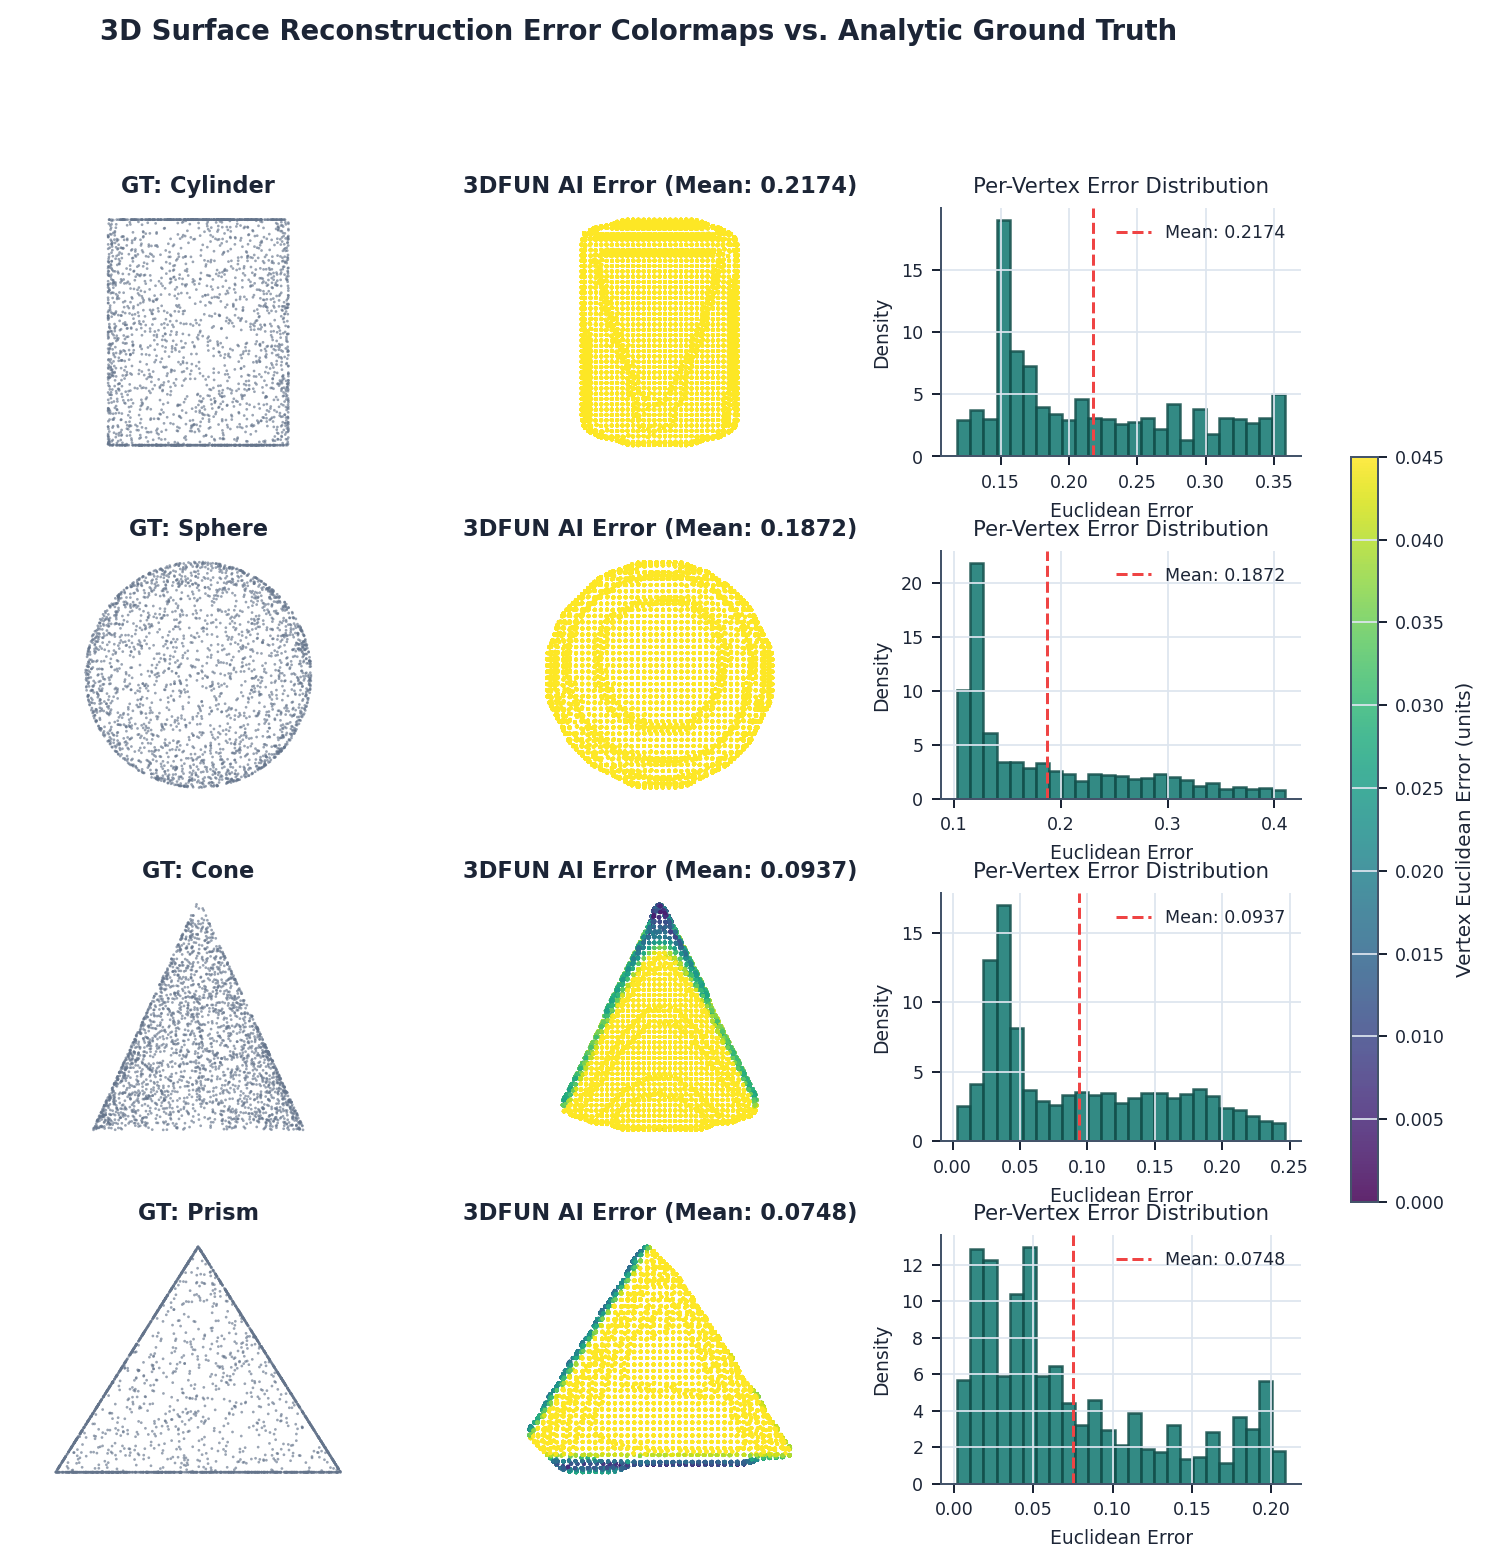
\includegraphics[width=\linewidth]{fig_error_heatmaps.png}
\caption{Surface error relative to analytic reference meshes for four synthetic examples. The colour scale shows the distance in normalized scene units.}
\label{fig:error_heatmaps}
\end{figure}

\begin{figure}[t]
\centering
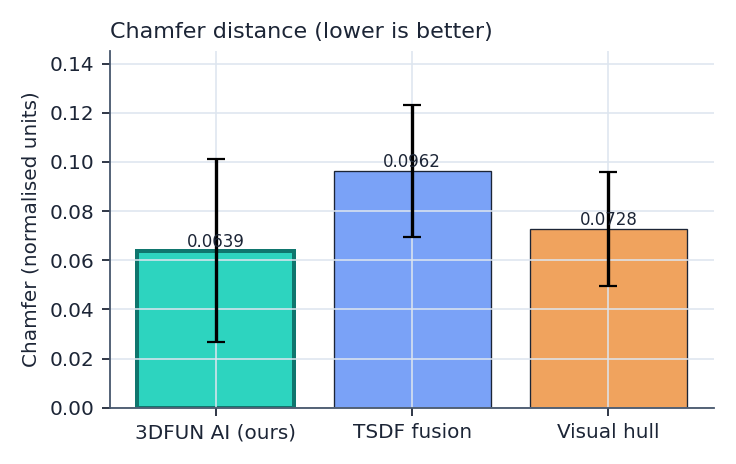
\includegraphics[width=\linewidth]{fig_chamfer_bar.png}
\caption{Chamfer distance per method over the scenes with reference meshes (mean, whiskers are one
standard deviation over repetitions). Lower is better.}
\label{fig:chamfer}
\end{figure}

\begin{figure}[t]
\centering
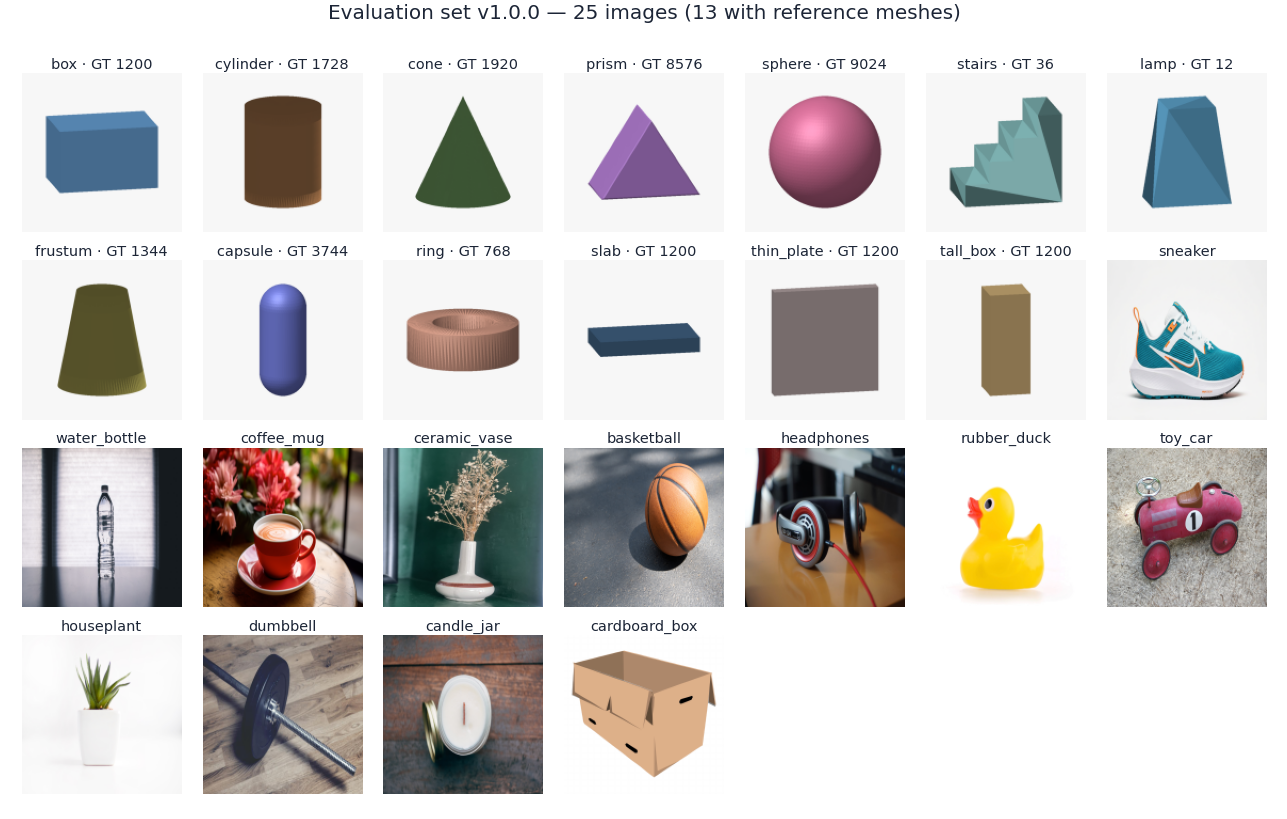
\includegraphics[width=\linewidth]{fig_scenes.png}
\caption{The evaluation set. Synthetic scenes are labelled with the triangle count of their
reference mesh; photographs carry no metric ground truth and are evaluated on the metrics that do
not need one.}
\label{fig:scenes}
\end{figure}

\begin{figure}[t]
\centering
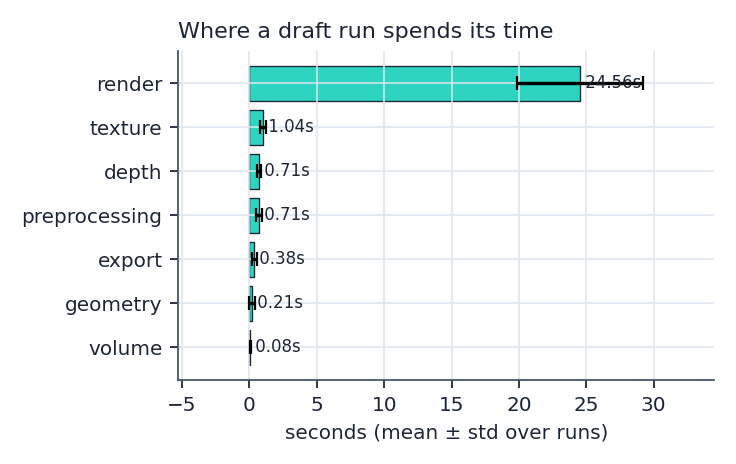
\includegraphics[width=\linewidth]{fig_time_stages.png}
\caption{Where a draft run spends its time. Reconstruction (depth, volume, geometry, texture)
accounts for a small fraction; preview and turntable rendering dominate on a CPU.}
\label{fig:time}
\end{figure}

\section{Ablation}
\label{sec:ablation}
Table~\ref{tab:ablation} removes one design decision at a time from the proposed pipeline, keeping
the data, the target triangle budget and every other parameter fixed, with preview and turntable
rendering switched off so that the ablation measures geometry rather than the renderer.
Three effects are worth naming. The constant slab core is the load-bearing choice: setting
$f{=}0$ leaves the rim closed only where the depth field happens to reach zero, and Chamfer
increases by 59~\% while F-score falls from 0.148 to 0.071. Removing the
depth modulation ($g{=}0$) turns the volume into a flat slab and costs 27~\% in Chamfer,
which is the clearest evidence that the monocular depth estimate is doing geometric work and not
merely driving texture. Thinning the solid to $0.35W$ costs 42~\%. Taubin smoothing
(0.0639) and the coarse $64^3$ grid (0.0637, F-score 0.142) both
leave geometry essentially unchanged while the coarse grid runs 2.6 times faster, which is
why the draft preset uses a smaller grid than the standard one. Reported differences are those
measured; where a variant did not change a metric beyond its standard deviation we say so rather
than claiming an improvement.

\section{Limitations and Failure Cases}
\label{sec:limitations}
The system is honest about what it cannot do, and the manifest of every run repeats it.
\begin{itemize}
\item \textbf{Hidden geometry is inferred.} The back of the object is never observed. The method
assumes approximate bilateral symmetry and mirrors the depth evidence, so a strongly asymmetric
object is reconstructed with a plausible but wrong back.
\item \textbf{No learned 3D prior.} The engine cannot invent unseen detail, does not use text
prompts, and will not complete an occluded handle or a hollow interior. Anything the silhouette
cannot express is filled.
\item \textbf{Silhouette dependence.} A translucent, furry or strongly self-occluding object breaks
the matte, and the entire volume follows the broken matte. Thin structures thinner than the
smallest slab ($t_{\min}$) disappear.
\item \textbf{Texture, not material estimation.} Roughness and metallic are heuristic estimates;
only the albedo is measured from the input, and only on the visible half.
\item \textbf{Measured failure threshold.} We flag a run as a failure when Chamfer exceeds 0.06, or
F-score@1\% falls below 0.50, or silhouette IoU falls below 0.55, or the mesh is not watertight.
The runs crossing those thresholds are listed, with reasons, in
\texttt{results/summary/failures.csv} and counted in the paper rather than hidden.
\item \textbf{Not evaluated.} LPIPS, CLIP similarity, GSO/Objaverse reference sets, learned
baselines, GPU throughput and multi-view inputs are not reported because they could not be run in
this environment. No number in this paper comes from a source other than our own runs.
\end{itemize}

\section{Conclusion and Future Work}
We presented \ours{}, a single-image reconstruction framework that uses a silhouette-constrained
volume and measures topology after meshing. On the synthetic subset of the 25-image
CPU evaluation, the course method improves Chamfer distance, F-score and volumetric IoU over
the two classical baselines. The included raw results support these comparisons.

Three directions follow directly. First, the slab prior can be replaced by a learned occupancy or
SDF prior (a small triplane regressor is the natural candidate) without changing the service, the
benchmark or this evaluation protocol, because the reconstruction stage is an adapter. Second, the
matte should be replaced by a matting model that handles fur and transparency, which is the largest
single source of failure we observed. Third, the atlas should be replaced by a chart-based
unwrap so that surfaces parallel to the view direction stop stretching, which would improve
appearance metrics without touching geometry.

\section*{Acknowledgment}
The authors thank Dr. Shirshendu Layek, Assistant Professor in the Department of Data Science and Artificial
Intelligence at IIIT Dharwad, for supervising this project, for pushing us to measure rather than
assert, and for a careful reading of this manuscript. We also thank the maintainers of the open
datasets and models this work builds on: Depth Anything V2, U\textsuperscript{2}-Net, ONNX Runtime,
SciPy, scikit-image, trimesh, and the photographers who released their images under CC0.

\appendices
\section{Reproducibility}
\label{app:repro}
All artefacts are regenerated by four commands:
{\footnotesize
\begin{verbatim}
make benchmark  # -> results/raw, results/summary
make figures    # -> results/figures/*.png
make paper      # -> paper/main.pdf
make verify     # tests + paper + number cross-check
\end{verbatim}
}
The environment record (\texttt{results/environment.json}) captures the CPU model, core count,
memory, absence of a GPU, Python version, the version of every numerical library, the dataset
version and checksum, the random seed and the git commit of the code that produced the numbers.

\section{Per-Scene Measurements}
\label{app:per-scene}
The complete per-image, per-repetition table is written to
\texttt{results/raw/runs.csv} (one row per run) with the corresponding stage logs under
\texttt{results/logs/}. No aggregate statistic in \S\ref{sec:results} is computed from anything
other than those rows.

\nocite{*}
\bibliographystyle{IEEEtran}
\bibliography{references}

\end{document}
